%! TEX TS-program = xelatex
%! TEX encoding = UTF-8 Unicode

\documentclass{article}
\usepackage{fontspec, graphicx}
\usepackage{hyperref}
\usepackage{mathtools}
\usepackage[a4paper, margin=1in]{geometry}

\graphicspath{ {images/}}

\setmainfont{DejaVuSansMono}



\begin{document}
	\title{ELEC3201 - Robotic Systems\\Notes}
	\author{Bradley Mason\\ University of Southampton}
	\maketitle
	\newpage
	
	\tableofcontents
	\newpage
	\section*{Tele-Robotics}
	\pagestyle{headings}
	\markright{L15 - Tele-Robotics\hfill 17/11/16 \hfill}
	\addcontentsline{toc}{section}{L15 - Tele-Robotics}
	{\bfseries Teleoperation} - To operate a vehicle or robotic system over a distance.\\
	The distance can vary from tens of centimetres to millions of kilometres but a person will always be in the loop.\\
	\\Motivation:
	\begin{itemize}
		\item The State of the Art - true AI is too difficult
		\item Remove humans from hazardous environments
		\item Reduce cost by not having man rated vahicles
	\end{itemize}
	{\bfseries Telepistemology} - Study of knowledge acquired at a distance\\
	\\Teleoperation systems are best suited for tasks that are unstructured and not repetitive. This is where the workspace cannot be engineered to permit the use of industrial manipulators, key portions of the task require a high degree of dexterous manipulations  (hand-eye coordination) but not continuously, and key key portions also require object recognition or situational awareness.\\
	The needs of the display technology do not exceed the limitations of the communication link (bandwidth, time delays). However it does not replace trained personnel.\\
	\\ The original tele-operated systems were master-slave systems based on mechanical pantographs developed by Argonne National Laboratory. They were developed for handling radioactive material ~1940s.\\
	\\In {\bfseries remote operations} the operator maintains visual contact with the robotic system. The control commands are then sent by either wire or radio, hence the operator does all the intelligent work but this has a limited range. Examples are drilling machines and switching locomotives.\\
	\\{\bfseries Human Supervisory Control} is split up into the following categories:\\
	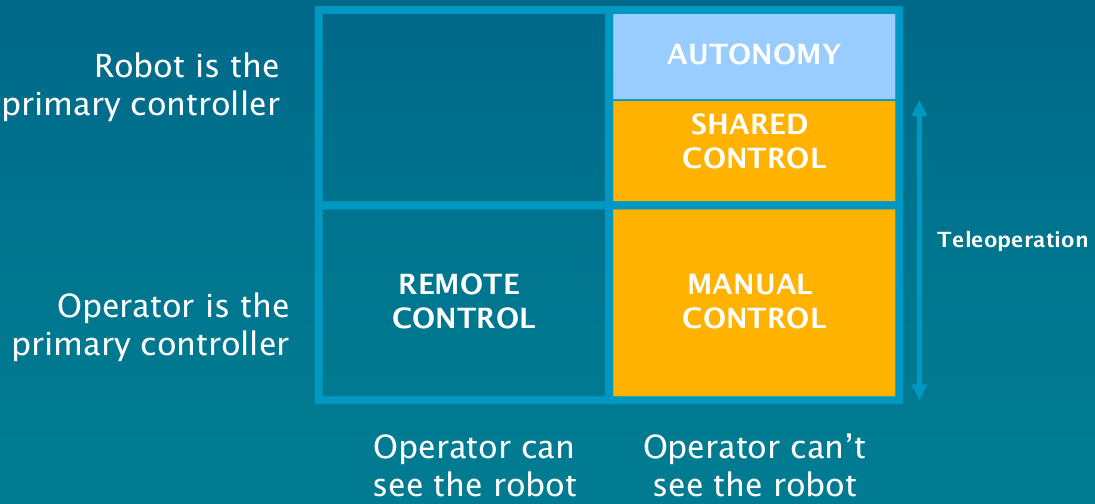
\includegraphics[scale=0.41]{human_supervisory_control}\\
	A {\bfseries Control Structure} has the structure where the local figure (human) contains the display and controls whereas the remote figure (robot) has sensors, control, effectors and drives. There is then communication between them. This must be considered at it will manage how much control the operator has and how much autonomy the robot has.\\ \\ \\
	\\{\bfseries Teleoperation} has two types:\\{\bfseries Closed loop control/Direct teleoperation}
	\begin{itemize}
		\item The operator controls the actuators by direct signals and gets real-time feedback
		\item This is possible only when the delay in the control loop are minimal
	\end{itemize}
	{\bfseries Coordinated teleoperation}
	\begin{itemize}
		\item The operator again controls the actuators but now there is some internal control - remote loop - included
		\item No autonomy included at the remote end
		\item The remote loops are used only to close these control loops that the operator is unable to control because of the delay
	\end{itemize}
	{\bfseries Supervisory Control}\\
	Human operators are intermittently giving directives and continually receiving information from a computer that itself closes an autonomous control loop through actuators and sensors in the task environment.\\
	This implies:
	\begin{itemize}
		\item Human is always involved, if only to set objectives
		\item Information may be the lack of information
		\item Computer is always involved
		\item Consider the impact of the command (compensate for time delays, inner loop control and safety reflexes)
	\end{itemize}
	{\bfseries Haptic Feedback} refers to technology which interfaces the user via the sense of touch by applying forces. vibrations and/or motions to the user.
	\\ \\
	There are many applications including medical (performing surgery remotely) and military (bomb disposal, rugged rc cars). There are plenty of ethical considerations to go along with this.\\
	There can be a problem of latency, anything below 0.5 seconds is considered acceptable and anything over that will create confusion. There have been ways around this such as with the mars rovers, they have no possibility for closed loops control so some autonomy is required. You used "move and wait" teleoperation where the robot has some self preservation rules to make up for the delay in human response time.\\
	There are of course other problems such as cognitive fatigue for the operator and situational awareness. There could be communications dropout or bandwidth issues. There are plenty of opportunities in digital systems for delays.\\ \\
	{\bfseries Telepresence} is where you use experience what the robot is sensing (VR, haptic feedback etc...). It improves human control adn can reduce simulator sickness by making the sensory feedback good enough to indice feeling of being present in the robot environment.
\end{document}